\chapter{THIẾT KẾ QUY TRÌNH NGHIỆP VỤ}
\label{ch:04}

\section{Lược đồ hoạt động quy trình Nhập kho}
Quy trình nhập kho bắt buộc thủ kho kiểm đếm quy cách trước khi gán vị trí ô kệ (Hình~\ref{fig:act_import}).

\begin{figure}[htbp]
    \centering
    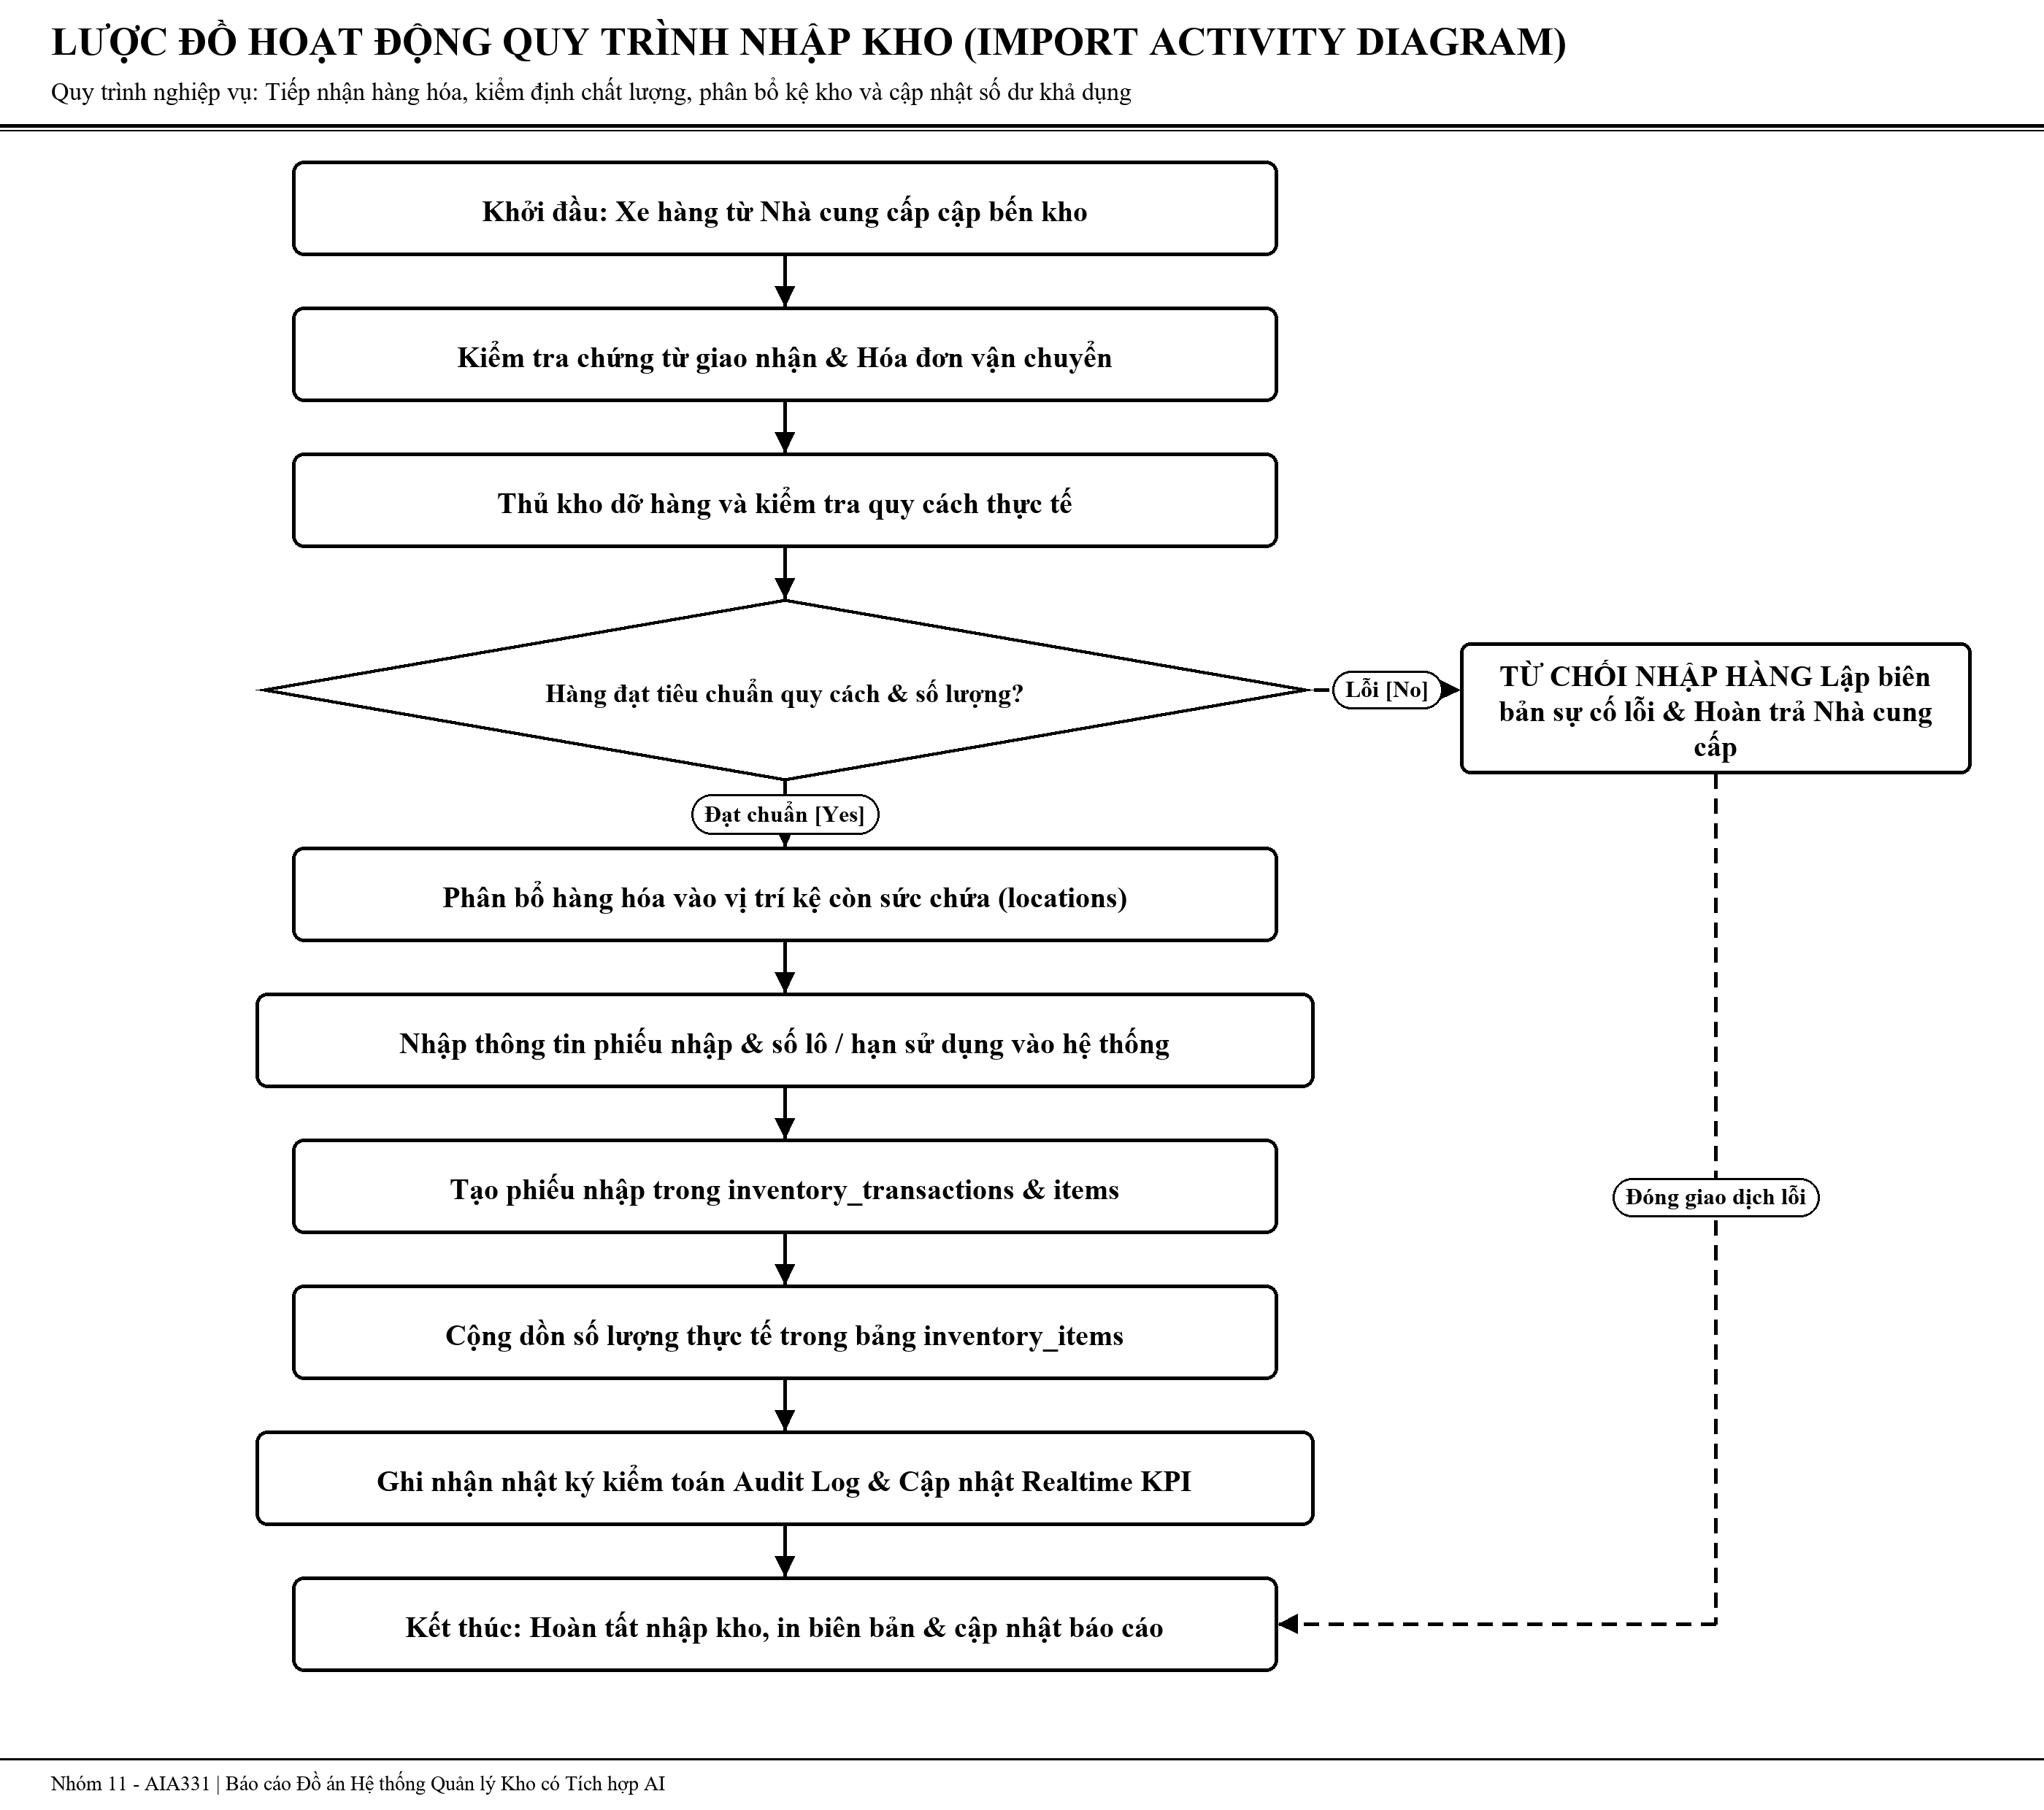
\includegraphics[width=0.85\textwidth]{04_luoc_do_hoat_dong_nhap_kho.png}
    \caption{Lược đồ hoạt động quy trình nghiệp vụ Nhập kho}
    \label{fig:act_import}
\end{figure}

\section{Lược đồ hoạt động quy trình Xuất kho}
Quy trình xuất kho kiểm tra số lượng tồn khả dụng để ngăn chặn xuất âm (Hình~\ref{fig:act_export}).

\begin{figure}[htbp]
    \centering
    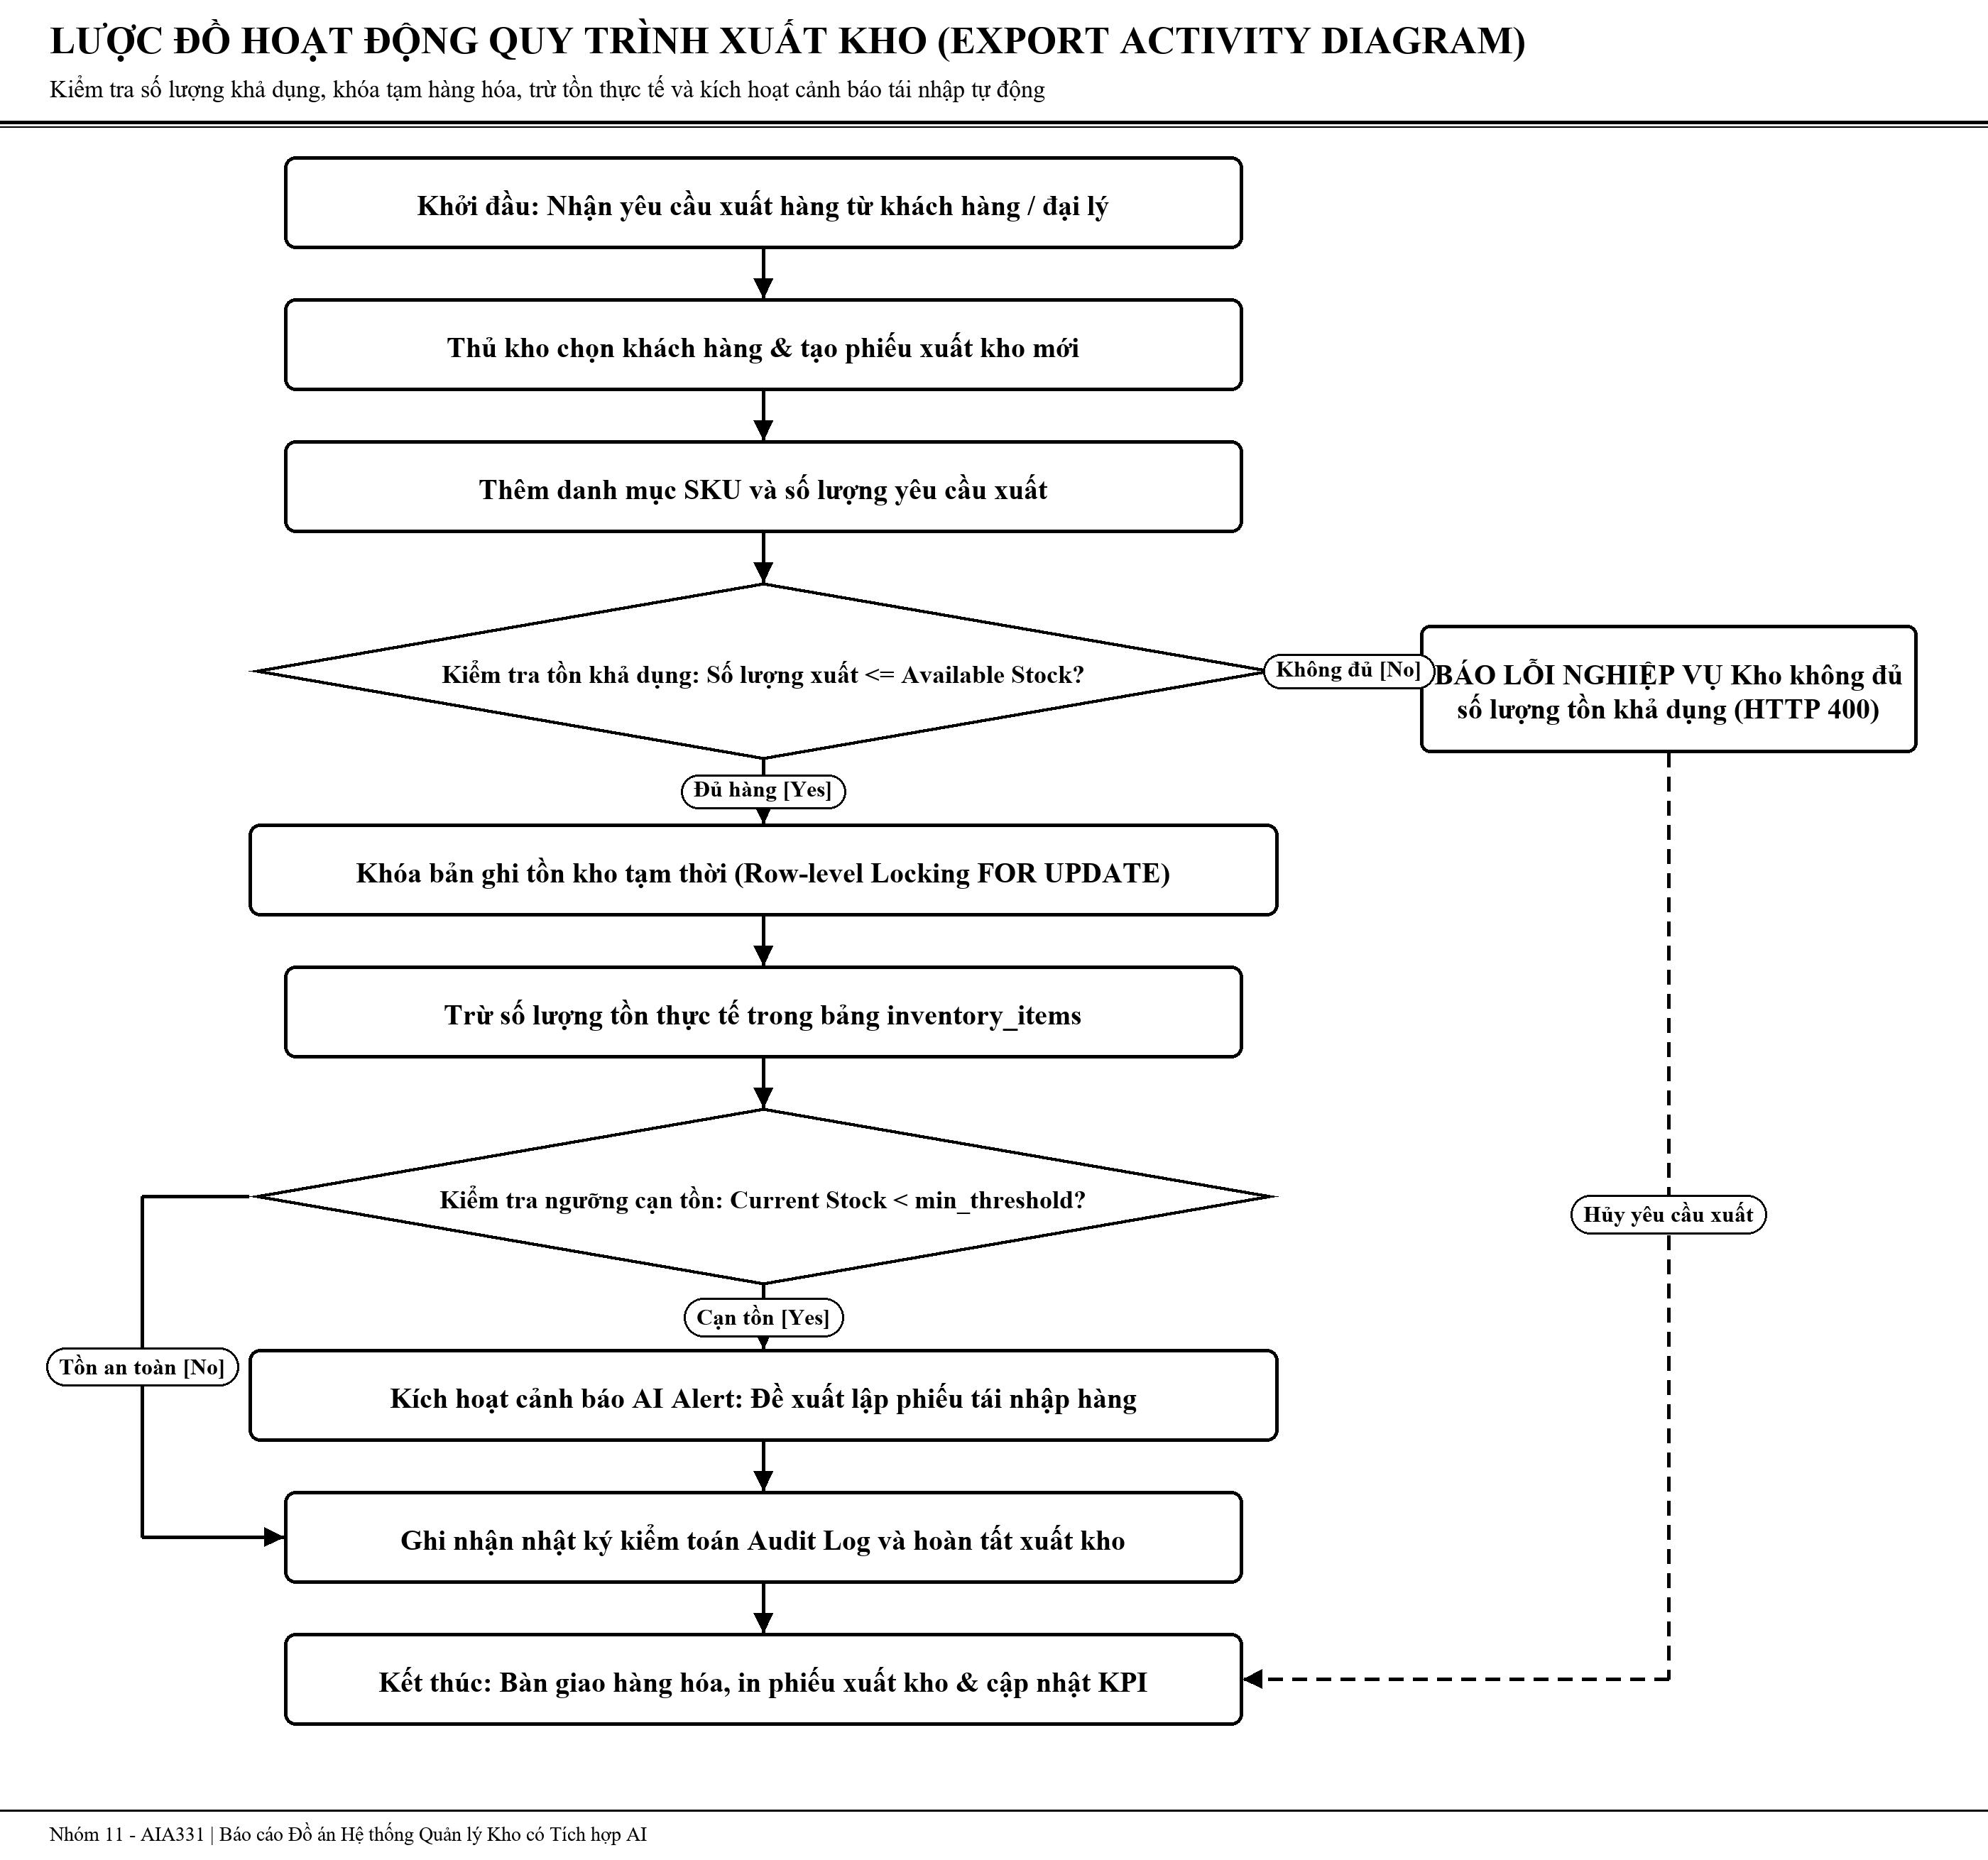
\includegraphics[width=0.85\textwidth]{05_luoc_do_hoat_dong_xuat_kho.png}
    \caption{Lược đồ hoạt động quy trình nghiệp vụ Xuất kho và kiểm tra tồn an toàn}
    \label{fig:act_export}
\end{figure}
